\documentclass{beamer}
\usepackage{graphicx}
\usepackage{tabularx}
\usepackage{listings}
\usepackage{xcolor}
\usepackage{amssymb}

% Theme and color scheme
\usetheme{Madrid}
\usecolortheme{seahorse}
\setbeamertemplate{itemize items}[square]

% Fix block colors - white text on blue blocks
\setbeamercolor{block title}{fg=white,bg=blue!75!black}
\setbeamercolor{block body}{fg=black,bg=blue!5!white}
\setbeamercolor{block title alerted}{fg=white,bg=red!75!black}
\setbeamercolor{block body alerted}{fg=black,bg=red!5!white}
\setbeamercolor{block title example}{fg=white,bg=green!50!black}
\setbeamercolor{block body example}{fg=black,bg=green!5!white}

% Fix outline text color
\setbeamercolor{section in toc}{fg=black}
\setbeamercolor{subsection in toc}{fg=black}

% Reduce font sizes
\setbeamerfont{block title}{size=\small}
\setbeamerfont{block body}{size=\small}
\setbeamerfont{footnote}{size=\tiny}
\setbeamerfont{caption}{size=\small}

% Title page information
\title{Multi-Frame Story Generation System}
\subtitle{Task 1: Story}
\author{Keyu HU \quad Siqi CHEN \quad Zhenzhuo LI}
\date{\today}

\begin{document}

% 1. Title Page
\frame{\titlepage}

% 2. Table of Contents
\begin{frame}{Outline}
    \tableofcontents
\end{frame}

% 3. Pipeline Overview
\section{PIPELINE}
\begin{frame}{PIPELINE: From Text to Multi-Frame Images}
    \begin{columns}
        \column{0.55\textwidth}
        \includegraphics[width=\textwidth,height=0.7\textheight,keepaspectratio]{images/case01_storyboard.png}
        \column{0.45\textwidth}
        \footnotesize
        \begin{itemize}
            \item \textbf{Input}: Raw Text scripts with \texttt{[SCENE-N]} and \texttt{<Name>} tags
            \item \textbf{Processing}: LLM Processor (3-phase analysis)
            \item \textbf{Output}: Storyboard images
        \end{itemize}
    \end{columns}
\end{frame}

\begin{frame}{System Architecture}
    \begin{columns}
        \column{0.55\textwidth}
        \footnotesize
        \textbf{Four-Layer Pipeline:}
        \begin{enumerate}
            \item \textbf{Script Director} (LLM Parser)
            \item \textbf{Asset Anchor} (Character Portraits)
            \item \textbf{Core Generator} (SDXL Pipeline)
            \item \textbf{Evaluation Hub} (CLIP + LPIPS)
        \end{enumerate}
        \column{0.45\textwidth}
        \begin{block}{Key Metrics (32 cases)}
            \footnotesize
            \begin{tabular}{lr}
                Avg CLIP Score & 0.288 \\
                Avg Consistency & 0.386 \\
                Success Rate & 100\% \\
            \end{tabular}
        \end{block}
    \end{columns}
\end{frame}

% 4. LLM Processor - Three Phases
\section{LLM PROCESSOR}
\subsection{Phase 1: Story Analysis}
\begin{frame}{Phase 1: Story Analysis}
    \footnotesize
    \begin{itemize}
        \item Character identification and unique ID assignment (e.g., \texttt{[Lily\_001]})
        \item Visual anchor extraction: clothing, hairstyle, color scheme
        \item Action decomposition per frame (e.g., ``stands by window'' $\rightarrow$ pose + environment)
    \end{itemize}
    \begin{block}{Example: Case 01 - Lily}
        \footnotesize
        \texttt{visual\_description: ``Young woman with auburn hair and round glasses, wearing a white blouse and black skirt.''}
    \end{block}
\end{frame}

\subsection{Phase 2: Prompt Generation}
\begin{frame}{Phase 2: Prompt Generation}
    \footnotesize
    \begin{itemize}
        \item Generate detailed SDXL prompts based on Phase 1 analysis
        \item Enforce cross-frame appearance consistency
        \item Multi-character scenes: LEFT/RIGHT spatial positioning
    \end{itemize}
    \begin{block}{Enhanced Prompt Structure}
        \footnotesize
        \texttt{[character\_token], [visual\_description], [action], [setting], [lighting], photorealistic, sharp focus}
    \end{block}
\end{frame}

\subsection{Phase 3: Refinement}
\begin{frame}{Phase 3: Refinement}
    \footnotesize
    \begin{itemize}
        \item Consistency verification (clothing drift detection)
        \item Pronoun resolution (he/she/they $\rightarrow$ specific character)
        \item Visual description prefix matching for character deduplication
    \end{itemize}
\end{frame}

% 5. Case Studies - Success Examples
\section{CASE STUDIES}
\begin{frame}{Case 11: Olivia in Classroom (Excellent Consistency)}
    \begin{columns}
        \column{0.65\textwidth}
        \includegraphics[width=\textwidth,height=0.75\textheight,keepaspectratio]{images/case11_storyboard.png}
        \column{0.35\textwidth}
        \footnotesize
        \textbf{Metrics:}
        \begin{itemize}
            \item CLIP: 0.331, Consistency: 0.420
            \item Overall: 0.367
        \end{itemize}
        \vspace{0.3em}
        \textbf{Achievements:}
        \begin{itemize}
            \item \checkmark Auburn hair maintained
            \item \checkmark Outfit consistent
            \item \checkmark Smooth transitions
        \end{itemize}
    \end{columns}
\end{frame}

\begin{frame}{Case 01: Lily Making Breakfast (Strong Facial Identity)}
    \begin{columns}
        \column{0.65\textwidth}
        \includegraphics[width=\textwidth,height=0.75\textheight,keepaspectratio]{images/case01_storyboard.png}
        \column{0.35\textwidth}
        \footnotesize
        \textbf{Metrics:}
        \begin{itemize}
            \item CLIP: 0.310, Consistency: 0.393
            \item Overall: 0.343
        \end{itemize}
        \vspace{0.3em}
        \textbf{Achievements:}
        \begin{itemize}
            \item \checkmark Round glasses preserved
            \item \checkmark Hair + outfit consistent
            \item \checkmark Kitchen setting maintained
        \end{itemize}
    \end{columns}
\end{frame}

\begin{frame}{Case 12: Ethan by the Sea (Scene Coherence)}
    \begin{columns}
        \column{0.65\textwidth}
        \includegraphics[width=\textwidth,height=0.75\textheight,keepaspectratio]{images/case12_storyboard.png}
        \column{0.35\textwidth}
        \footnotesize
        \textbf{Metrics:}
        \begin{itemize}
            \item CLIP: 0.288, Consistency: 0.360
            \item Overall: 0.317
        \end{itemize}
        \vspace{0.3em}
        \textbf{Achievements:}
        \begin{itemize}
            \item \checkmark Beach environment consistent
            \item \checkmark Ocean lighting maintained
            \item \checkmark Walking motion coherent
        \end{itemize}
    \end{columns}
\end{frame}

\begin{frame}{Extra 02: Mark Riding Bike (Dynamic Scene)}
    \begin{columns}
        \column{0.65\textwidth}
        \includegraphics[width=\textwidth,height=0.75\textheight,keepaspectratio]{images/extra02_storyboard.png}
        \column{0.35\textwidth}
        \footnotesize
        \textbf{Metrics:}
        \begin{itemize}
            \item CLIP: 0.272, Consistency: 0.365
            \item Overall: 0.309
        \end{itemize}
        \vspace{0.3em}
        \textbf{Achievements:}
        \begin{itemize}
            \item \checkmark Outdoor transitions smooth
            \item \checkmark Time of day consistent
            \item \checkmark Action progression clear
        \end{itemize}
    \end{columns}
\end{frame}

% 6. Evaluation Metrics
\section{EVALUATION}
\begin{frame}{Quantitative Results (Selected Cases)}
    \footnotesize
    \begin{table}
        \begin{tabular}{|l|c|c|c|c|}
            \hline
            \textbf{Case} & \textbf{Character} & \textbf{CLIP} & \textbf{Consistency} & \textbf{Overall} \\
            \hline
            01 & Lily & 0.310 & 0.393 & 0.343 \\
            \hline
            11 & Olivia & 0.331 & 0.420 & 0.367 \\
            \hline
            12 & Ethan & 0.288 & 0.360 & 0.317 \\
            \hline
            Extra 02 & Mark & 0.272 & 0.365 & 0.309 \\
            \hline
            06 & Jack + Sara & 0.288 & 0.389 & 0.328 \\
            \hline
            03 & Cat + Dog & 0.295 & 0.378 & 0.329 \\
            \hline
        \end{tabular}
    \end{table}
    \vspace{0.5em}
    \tiny CLIP: text-image alignment (target $\geq$0.25) | LPIPS: inter-frame consistency (target $\geq$0.30)
\end{frame}

\begin{frame}{Metrics Explanation}
    \footnotesize
    \begin{block}{CLIP Score (Text-Image Alignment)}
        \footnotesize
        Measures how well generated images match the text prompts using OpenCLIP ViT-L-14. Target: $\geq$ 0.25
    \end{block}
    \begin{block}{LPIPS Consistency (Inter-Frame Identity)}
        \footnotesize
        Perceptual similarity between consecutive frames. Target: $\geq$ 0.30
    \end{block}
    \begin{block}{Overall Score}
        \footnotesize
        $0.6 \times \text{CLIP} + 0.4 \times \text{Consistency}$
    \end{block}
\end{frame}

% 7. Limitations
\section{LIMITATIONS}
\begin{frame}{Case 03: Cat + Dog - Animal Consistency Challenge}
    \begin{columns}
        \column{0.65\textwidth}
        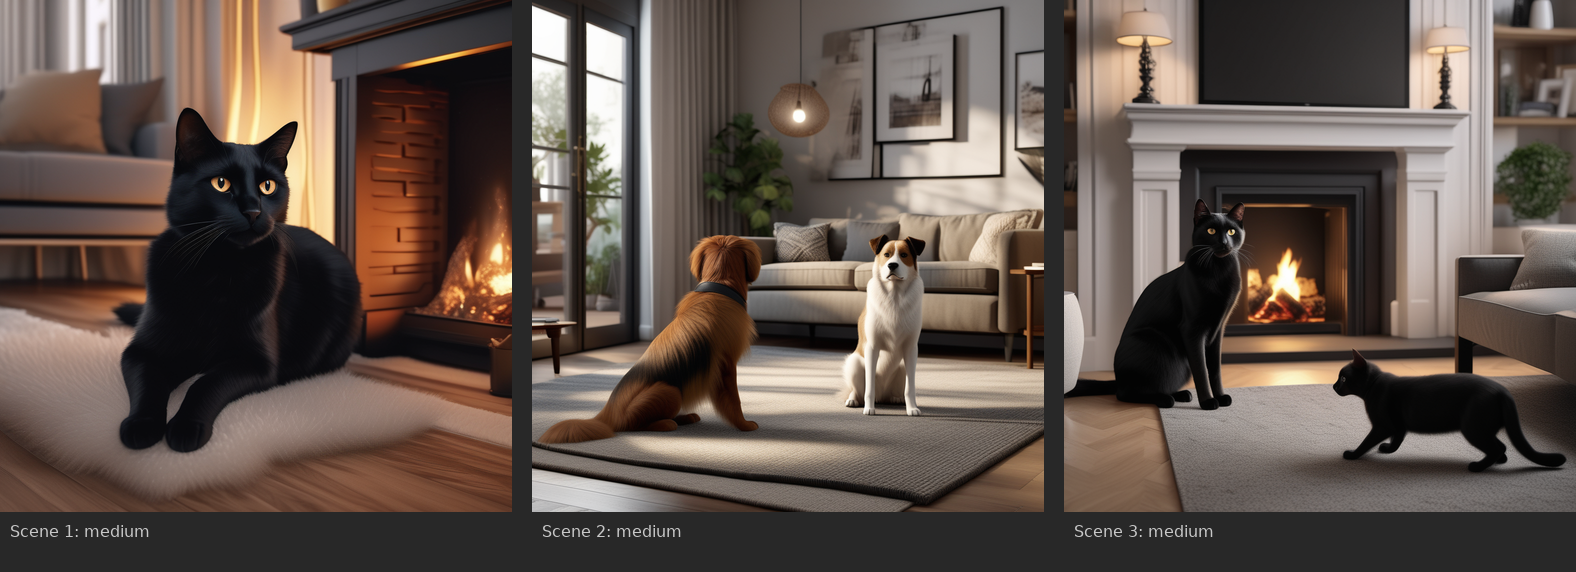
\includegraphics[width=\textwidth,height=0.75\textheight,keepaspectratio]{images/case03_storyboard.png}
        \column{0.35\textwidth}
        \footnotesize
        \textbf{Metrics:}
        \begin{itemize}
            \item CLIP: 0.295, Consistency: 0.378
            \item Overall: 0.329
        \end{itemize}
        \vspace{0.3em}
        \textbf{Challenges:}
        \begin{itemize}
            \item \textbf{Animal features inconsistent}
            \item Multi-character tracking difficult
            \item Scene transitions jarring
        \end{itemize}
    \end{columns}
\end{frame}

\begin{frame}{Case 06: Jack + Sara - Multi-Character Consistency}
    \begin{columns}
        \column{0.65\textwidth}
        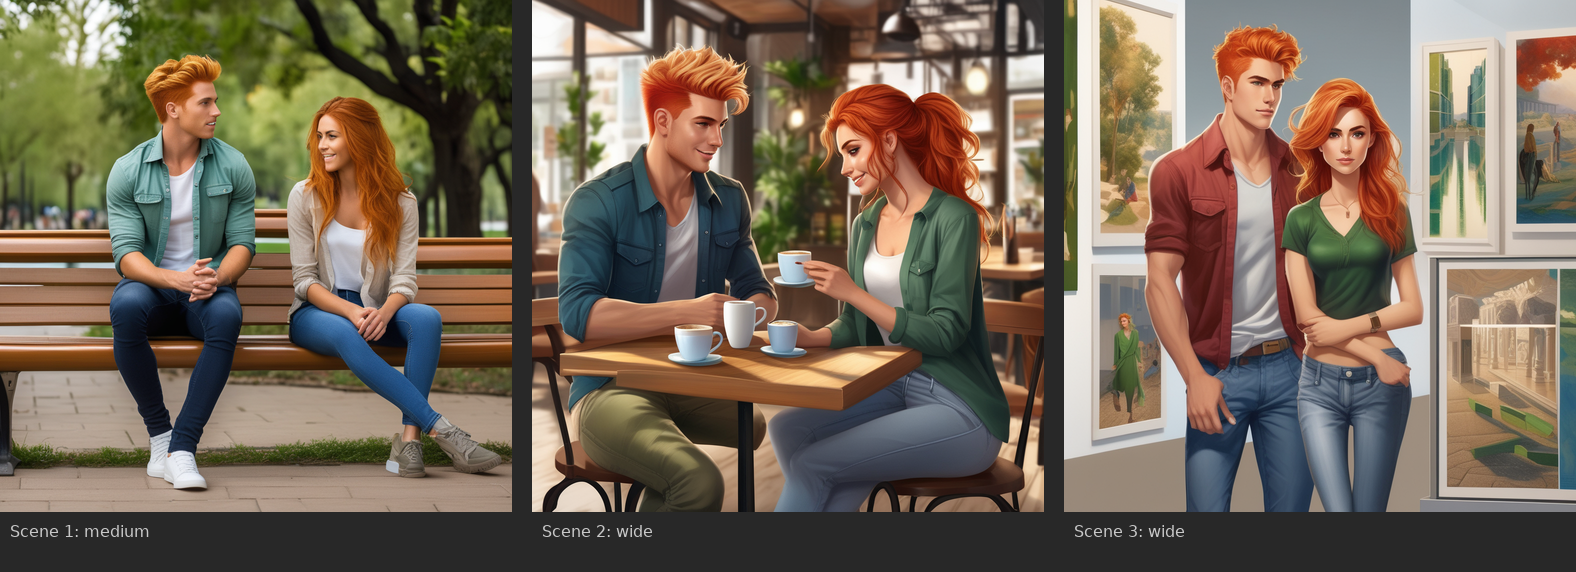
\includegraphics[width=\textwidth,height=0.75\textheight,keepaspectratio]{images/case06_storyboard.png}
        \column{0.35\textwidth}
        \footnotesize
        \textbf{Metrics:}
        \begin{itemize}
            \item CLIP: 0.288, Consistency: 0.389
            \item Overall: 0.328
        \end{itemize}
        \vspace{0.3em}
        \textbf{Challenges:}
        \begin{itemize}
            \item \textbf{Clothing changes between scenes}
            \item LEFT/RIGHT positioning unstable
            \item Face identity drift
        \end{itemize}
    \end{columns}
\end{frame}

\begin{frame}{Case 13: Robot - Abstract Character Misidentification}
    \begin{columns}
        \column{0.65\textwidth}
        \includegraphics[width=\textwidth,height=0.75\textheight,keepaspectratio]{images/case13_storyboard.png}
        \column{0.35\textwidth}
        \footnotesize
        \textbf{Metrics:}
        \begin{itemize}
            \item CLIP: 0.205, Consistency: 0.377
            \item Overall: 0.274
        \end{itemize}
        \vspace{0.3em}
        \textbf{Challenges:}
        \begin{itemize}
            \item \textbf{Robot generated as human}
            \item No metallic body features
            \item Prompt override by SDXL priors
        \end{itemize}
    \end{columns}
\end{frame}

\begin{frame}{Summary of Limitations}
    \begin{columns}
        \column{0.5\textwidth}
        \footnotesize
        \textbf{Challenges:}
        \begin{itemize}
            \item \textbf{Animal characters}: Inconsistent features
            \item \textbf{Multi-character}: Clothing/position drift
            \item \textbf{Abstract entities}: Robots $\rightarrow$ humans
        \end{itemize}
        \column{0.5\textwidth}
        \footnotesize
        \textbf{Strengths:}
        \begin{itemize}
            \item \checkmark Human facial identity
            \item \checkmark Scene/setting consistency
            \item \checkmark Single character stories
            \item \checkmark Lighting and mood
        \end{itemize}
    \end{columns}
\end{frame}

% 8. Future Work
\section{FUTURE WORK}
\begin{frame}{Future Work}
    \begin{columns}
        \column{0.5\textwidth}
        \footnotesize
        \textbf{Character Consistency:}
        \begin{itemize}
            \item Integrate IP-Adapter or ControlNet for stronger anchoring
            \item Implement cross-frame attention (ReDiStory, ICSA)
            \item Face embedding-based consistency loss
        \end{itemize}
        \column{0.5\textwidth}
        \footnotesize
        \textbf{Non-Human Characters:}
        \begin{itemize}
            \item Specialized prompts for animals/robots
            \item Fine-tune SDXL on non-human entities
            \item Reference image conditioning
        \end{itemize}
    \end{columns}
    \vspace{1em}
    \begin{block}{Long-term Vision}
        \footnotesize
        Video generation with temporal consistency; TTS integration for narrated stories
    \end{block}
\end{frame}

% 9. Q&A
\section{Q\&A}
\begin{frame}{Questions \& Discussion}
    \begin{center}
        \LARGE Thank You! \\
        \vspace{1em}
        \large Questions?
    \end{center}
    \vspace{1em}
    \begin{block}{Key Contributions}
        \footnotesize
        \begin{itemize}
            \item LLM-driven script parsing with visual anchor extraction
            \item CLIP-based character portrait anchoring
            \item Compressed visual memory bank for consistency
            \item Quantitative evaluation pipeline (CLIP + LPIPS)
        \end{itemize}
    \end{block}
\end{frame}

% 10. Backup Slides
\section{BACKUP}
\begin{frame}{Pipeline Flow Diagram}
    \begin{columns}
        \column{0.6\textwidth}
        \includegraphics[width=\textwidth,height=0.85\textheight,keepaspectratio]{images/case01_storyboard.png}
        \column{0.4\textwidth}
        \footnotesize
        \textbf{Pipeline Steps:}
        \begin{enumerate}
            \item Input: \texttt{[SCENE-1] <Lily> makes breakfast}
            \item LLM Parser: Extract character + generate prompt
            \item SDXL Generation: 3 frames
            \item Output: Storyboard + metrics
        \end{enumerate}
    \end{columns}
\end{frame}

\begin{frame}{Technical Details: Character Portrait Generation}
    \begin{columns}
        \column{0.5\textwidth}
        \footnotesize
        \textbf{Portrait Pipeline:}
        \begin{enumerate}
            \item Extract visual\_description from LLM
            \item Generate portrait using SDXL txt2img
            \item Extract CLIP features using ViT-L-14
            \item Store for cross-frame consistency
        \end{enumerate}
        \column{0.5\textwidth}
        \footnotesize
        \textbf{Memory Bank:}
        \begin{itemize}
            \item Compressed visual features (128-dim)
            \item Importance-weighted retrieval
            \item Temporal decay (0.9 factor)
        \end{itemize}
    \end{columns}
\end{frame}

\end{document}
